%% Este documento foi baseado no abtex2-modelo-trabalho-academico.tex, v-1.9.3 laurocesar
%% abnTeX2 group at http://abntex2.googlecode.com/ 
% ------------------------------------------------------------------------
% ------------------------------------------------------------------------
% Monografia de Ciencia da Computacao da Universidade Paulista - UNIP
% ------------------------------------------------------------------------
% ------------------------------------------------------------------------

\documentclass[
	% -- opções da classe memoir --
	12pt,				% tamanho da fonte
	openright,			% capítulos começam em pág ímpar (insere página vazia caso preciso)
	twoside,			% para impressão em verso e anverso. Oposto a oneside
	a4paper,			% tamanho do papel. 
	% -- opções da classe abntex2 --
	%chapter=TITLE,		% títulos de capítulos convertidos em letras maiúsculas
	%section=TITLE,		% títulos de seções convertidos em letras maiúsculas
	%subsection=TITLE,	% títulos de subseções convertidos em letras maiúsculas
	%subsubsection=TITLE,% títulos de subsubseções convertidos em letras maiúsculas
	% -- opções do pacote babel --
	english,			% idioma adicional para hifenização
	french,				% idioma adicional para hifenização
	spanish,			% idioma adicional para hifenização
	brazil				% o último idioma é o principal do documento
	]{abntex2}

% ---
% Pacotes básicos 
% ---
\usepackage{lmodern}			% Usa a fonte Latin Modern			
\usepackage[T1]{fontenc}		% Selecao de codigos de fonte.
\usepackage[utf8]{inputenc}		% Codificacao do documento (conversão automática dos acentos)
\usepackage{lastpage}			% Usado pela Ficha catalográfica
\usepackage{indentfirst}		% Indenta o primeiro parágrafo de cada seção.
\usepackage{color}				% Controle das cores
\usepackage{graphicx}			% Inclusão de gráficos
\usepackage{microtype} 			% para melhorias de justificação
% ---
		
% ---
% Pacotes adicionais, usados apenas no âmbito do Modelo Canônico do abnteX2
% ---
\usepackage{lipsum}				% para geração de dummy text
% ---

% ---
% Pacotes de citações
% ---
\usepackage[brazilian,hyperpageref]{backref}	 % Paginas com as citações na bibl
\usepackage[alf]{abntex2cite}	% Citações padrão ABNT

% --- 
% CONFIGURAÇÕES DE PACOTES
% --- 

% ---
% Configurações do pacote backref
% Usado sem a opção hyperpageref de backref
\renewcommand{\backrefpagesname}{Citado na(s) página(s):~}
% Texto padrão antes do número das páginas
\renewcommand{\backref}{}
% Define os textos da citação
\renewcommand*{\backrefalt}[4]{
	\ifcase #1 %
		Nenhuma citação no texto.%
	\or
		Citado na página #2.%
	\else
		Citado #1 vezes nas páginas #2.%
	\fi}%
% ---

% ---
% Informações de dados para CAPA e FOLHA DE ROSTO
% ---
\titulo{Desenvolvimento de Portal Facilitador de Acesso a Dados Governamentais Abertos}
\autor{Kerolláine Lauto de Oliveira}
\local{Brasil}
\data{2015}
\orientador{Danielle Bentivoglio Colturato}
%\coorientador{Equipe \abnTeX}
\instituicao{%
  Universidade Paulista -- UNIP
  \par
  Instituto de Ciências Exatas e Tecnologia
  \par
  Ciência da Computação}
\tipotrabalho{Monografia (Graduação)}
% O preambulo deve conter o tipo do trabalho, o objetivo, 
% o nome da instituição e a área de concentração 
\preambulo{Pesquisa sobre os dados governamentais abertos no Brasil, assim como o desenvolvimento de um portal sobre as
proposições tramitadas no Congresso Nacional.}
% ---


% ---
% Configurações de aparência do PDF final

% alterando o aspecto da cor azul
\definecolor{blue}{RGB}{41,5,195}

% informações do PDF
\makeatletter
\hypersetup{
     	%pagebackref=true,
		pdftitle={\@title}, 
		pdfauthor={\@author},
    	pdfsubject={\imprimirpreambulo},
	    pdfcreator={LaTeX with abnTeX2},
		pdfkeywords={abnt}{latex}{abntex}{abntex2}{trabalho acadêmico}, 
		colorlinks=true,       		% false: boxed links; true: colored links
    	linkcolor=blue,          	% color of internal links
    	citecolor=blue,        		% color of links to bibliography
    	filecolor=magenta,      		% color of file links
		urlcolor=blue,
		bookmarksdepth=4
}
\makeatother
% --- 

% --- 
% Espaçamentos entre linhas e parágrafos 
% --- 

% O tamanho do parágrafo é dado por:
\setlength{\parindent}{1.3cm}

% Controle do espaçamento entre um parágrafo e outro:
\setlength{\parskip}{0.2cm}  % tente também \onelineskip

% ---
% compila o indice
% ---
\makeindex
% ---

% ----
% Início do documento
% ----
\begin{document}

% Seleciona o idioma do documento (conforme pacotes do babel)
%\selectlanguage{english}
\selectlanguage{brazil}

% Retira espaço extra obsoleto entre as frases.
\frenchspacing 

% ----------------------------------------------------------
% ELEMENTOS PRÉ-TEXTUAIS
% ----------------------------------------------------------
% \pretextual

% ---
% Capa
% ---
\imprimircapa
% ---

% ---
% Folha de rosto
% (o * indica que haverá a ficha bibliográfica)
% ---
\imprimirfolhaderosto*
% ---

% ---
% Inserir a ficha bibliografica
% ---

% Isto é um exemplo de Ficha Catalográfica, ou ``Dados internacionais de
% catalogação-na-publicação''. Você pode utilizar este modelo como referência. 
% Porém, provavelmente a biblioteca da sua universidade lhe fornecerá um PDF
% com a ficha catalográfica definitiva após a defesa do trabalho. Quando estiver
% com o documento, salve-o como PDF no diretório do seu projeto e substitua todo
% o conteúdo de implementação deste arquivo pelo comando abaixo:
%
% \begin{fichacatalografica}
%     \includepdf{fig_ficha_catalografica.pdf}
% \end{fichacatalografica}

\begin{fichacatalografica}
	\sffamily
	\vspace*{\fill}					% Posição vertical
	\begin{center}					% Minipage Centralizado
	\fbox{\begin{minipage}[c][8cm]{13.5cm}		% Largura
	\small
	%\imprimirautor
	Oliveira, Kerolláine Lauto.
	
	\hspace{0.5cm} \imprimirtitulo  / \imprimirautor. --
	\imprimirlocal, \imprimirdata-
	
	%\hspace{0.5cm} \pageref{LastPage} p. : il. (algumas color.) ; 30 cm.\\
	
	\hspace{0.5cm} \imprimirorientadorRotulo~\imprimirorientador\\
	
	\hspace{0.5cm}
	\parbox[t]{\textwidth}{\imprimirtipotrabalho~--~\imprimirinstituicao,
	\imprimirdata.}\\
	
	\hspace{0.5cm}
		1. Desenvolvimento Web.
		2. Dados governamentais abertos.
		2. Lei de acesso à Informação..
		I. Orientadora Danielle Bentivoglio Colturato.
		II. Universidade Paulista - UNIP.
		III. Instituto de Ciências Exatas e Tecnologia
		IV. Desenvolvimento de Portal Facilitador de Acesso a Dados Governamentais Abertos 			
	\end{minipage}}
	\end{center}
\end{fichacatalografica}
% ---

% ---

% ---
% Inserir folha de aprovação
% ---

% Isto é um exemplo de Folha de aprovação, elemento obrigatório da NBR
% 14724/2011 (seção 4.2.1.3). Você pode utilizar este modelo até a aprovação
% do trabalho. Após isso, substitua todo o conteúdo deste arquivo por uma
% imagem da página assinada pela banca com o comando abaixo:
%
% \includepdf{folhadeaprovacao_final.pdf}
%
\begin{folhadeaprovacao}

  \begin{center}
    {\ABNTEXchapterfont\large\imprimirautor}

    \vspace*{\fill}\vspace*{\fill}
    \begin{center}
      \ABNTEXchapterfont\bfseries\Large\imprimirtitulo
    \end{center}
    \vspace*{\fill}
    
    \hspace{.45\textwidth}
    \begin{minipage}{.5\textwidth}
        \imprimirpreambulo
    \end{minipage}%
    \vspace*{\fill}
   \end{center}
        
   Trabalho aprovado. \imprimirlocal, Junho de 2015:

   \assinatura{\textbf{\imprimirorientador} \\ Orientadora} 
   \assinatura{\textbf{Professor} \\ Convidado 1}
   \assinatura{\textbf{Professor} \\ Convidado 2}
   %\assinatura{\textbf{Professor} \\ Convidado 3}
   %\assinatura{\textbf{Professor} \\ Convidado 4}
      
   \begin{center}
    \vspace*{0.5cm}
    {\large\imprimirlocal}
    \par
    {\large\imprimirdata}
    \vspace*{1cm}
  \end{center}
  
\end{folhadeaprovacao}
% ---

% ---
% Dedicatória
% ---
\begin{dedicatoria}
   \vspace*{\fill}
   \centering
   \noindent
   \textit{ Este trabalho é dedicado à todos aqueles que,\\
   assim como eu, acreditam no poder do acesso à informação.} \vspace*{\fill}
\end{dedicatoria}
% ---

% ---
% Agradecimentos
% ---
\begin{agradecimentos}
 Agradeço a minha família que me incentiva e oferece o suporte necessário para eu possa alcançar todos os meus planos e 
 objetivos, e me ensinou desde cedo que tudo é tangível se trabalharmos para isso. Agradeço o meu noivo que sempre se 
 manteve ao meu lado com toda paciência e determinação do mundo, me motivando e ajudando sempre que necessário. Obrigada 
 por tudo.

Agradeço a todos os docentes pela rica experiência que me proporcionaram durante todos esses anos, permitindo que eu aprendesse
não somente sobre computação, mas que eu levasse comigo um pouco da experiência de vida e opiniões de cada um.

E também agradeço aos meus amigos, pela união e perseverança de sempre.
\end{agradecimentos}
% ---
 
% ---
% Epígrafe
% ---
\begin{epigrafe}
    \vspace*{\fill}
	\begin{flushright}
		\textit{`É difícil imaginar o poder que teremos com \\
		essa quantidade tão grande de tipos \\
		de dados diferentes que estão disponíveis.'\\
		(Tim Berners-Lee) Tradução nossa}
	\end{flushright}
\end{epigrafe}
% ---

% ---
% RESUMOS
% ---

% resumo em português
\setlength{\absparsep}{18pt} % ajusta o espaçamento dos parágrafos do resumo
\begin{resumo}

Dados são abertos quando qualquer coisa pode livremente usá-los, reutilizá-los e redistribuí-los sendo necessário, 
no máximo, creditar a sua autoria e compartilhar pela mesma licença. Dados governamentais abertos é a disponibilização,
através da \emph{web}, de informações e dados governamentais de domínio público para a livre utilização pela sociedade. Tais dados 
devem seguir oito princípios definidos por um grupo de trabalho denominado OpenGovData, e utilizar padrões da Web Semântica 
para tornar os dados significativos também para as máquinas. O Brasil faz parte da Parceira para o Governo Aberto, onde mais 
de 60 países tem o compromisso de fortalecer práticas relacionadas à transparência dos dados governamentais, entre outros. Em 
2011 também foi aprovada a Lei de Acesso à Informação, o que consequentemente possibilitou a criação do Portal Brasileiro de 
Dados Abertos. Desde então muitos portais do governo foram reformulados mas as informações são apenas disponibilizadas e não
processadas, evidenciando uma otimização necessária para obter resultados mais relevantes de determinado conjunto de dados. 
Nesse sentido, o objetivo deste trabalho é a utilização de tecnologia da informação para beneficiar a sociedade com a recente
abertura de dados governamentais compreendidos por máquinas. O subconjunto de dados utilizado para o projeto foi disponbilizado
pela Câmara dos Deputados e contém os dados referentes às proposições que tramitaram ou tramitam no Congresso Nacional. Foram
encontradas algumas dificuldades como, por exemplo, falta de padronização do conjunto de dados analisado e informações 
indisponíveis no site governamental. O portal, composto por ferramentas gŕaficas, um buscador de proposições e um sistema de 
votação, permite à sociedade encontrar novas informações e resultados a partir dos dados abertos utilizados.

 \textbf{Palavras-chave}: desenvolvimento web. dados governamentais abertos. acesso a informação. web semântica.
\end{resumo}

% resumo em inglês
\begin{resumo}[Abstract]
 \begin{otherlanguage*}{english}
\emph{ Data are "open" when anything can freely use, reuse and
redistribute it, needing only to give appropriate credits 
and share the same license.
Open government data is the disponibilization, in the web,
of public domain information and government data for anyone
in the society to use.
Such data must follow eight principles defined by a work group
denominated OpenGovData, and use Semantic Web standards to
prepare the data to machine consumption in addition to human consumption.
Brazil is a member of the Open Government Partnership, a group
of more than 60 countries commited to solidify practices related
to government data transparency, among other things.
In 2011 was approved the Information Access Act (english for Lei
de Acesso à Informação, LAI), responsible for the development of
the Brazilian Open Data Portal.
Since then, much of the existing government portals were reformulated,
but the data isn't processed and thought to be user friendly, bringing
up the need to analyse and to classify the data in order to create
valuable data to the society.
With this in mind, the main goal of this paper is to show a way
to use information technology to benefit the society with the
recent "opening" in government data policies.
The subset of data used in this paper's project is made available
by the Brazilian House of Representatives, containing information
about the law proposals, from past and current years.
Some difficulties has been found, such as, lack of standardization
of the chosen dataset and poor official documentation.
The portal, composed by graphic tools, a proposal finder and a voting system,
allows the society to find new information and results based of the raw
dataset.}
   \vspace{\onelineskip}
 
   \noindent 
   \emph{ \textbf {Keywords}: Web Development. government data. Information Access. Semantic Web.} 
 \end{otherlanguage*}
\end{resumo}

% ---

% ---
% inserir lista de ilustrações
% ---
\pdfbookmark[0]{\listfigurename}{lof}
\listoffigures*
\cleardoublepage
% ---

% ---
% inserir lista de tabelas
% ---
\pdfbookmark[0]{\listtablename}{lot}
\listoftables*
\cleardoublepage
% ---

% ---
% inserir lista de abreviaturas e siglas
% ---
\begin{siglas}
  \item[CSV] Comma-Separated Values
  \item[DGA] Dados Governamentais Abertos
  \item[DOU] Diário Oficial da União
  \item[JSON] JavaScript Object Notation (Notação de Objetos JavaScript)
  \item[SPARQL] SPARQL Protocol and RDF Query Language SPARQL
  \item[SOAP] Simple Object Access Protocol (Protocolo Simples de Acesso à Objetos)
  \item[WSDL] Web Services Description Language
  \item[UDDI] Universal Description, Discovery and Integration
  \item[W3C] World Wide Web Consortium, empresa de padronização da \emph{internet}
  \item[XML] eXtensible Markup Language
\end{siglas}
% ---

% ---
% inserir lista de símbolos
% ---
%\begin{simbolos}
%  \item[$ \Gamma $] Letra grega Gama
%  \item[$ \Lambda $] Lambda
%  \item[$ \zeta $] Letra grega minúscula zeta
%  \item[$ \in $] Pertence
%\end{simbolos}
% ---

% ---
% inserir o sumario
% ---
\pdfbookmark[0]{\contentsname}{toc}
\tableofcontents*
\cleardoublepage
% ---



% ----------------------------------------------------------
% ELEMENTOS TEXTUAIS
% ----------------------------------------------------------
\textual

% ----------------------------------------------------------
% Introdução
% ----------------------------------------------------------
\chapter[Introdução]{Introdução}
% ----------------------------------------------------------

A quantidade de informações disponibilizadas com a Lei de Acesso à Informação cresce exponencialmente, juntamente com o alcance
e poder de tal. 
Não seria diferente com dados públicos. O Brasil faz parte da \citeonline{ParceriaGA} onde, segundo a \citeonline{CGUGA}, mais 
de 60 países tem o compromisso de fortalecer práticas relacionadas à transparência dos atos governamentais, prevenir e 
combater a corrupção, melhorar a prestação do serviço público e promover o acesso à informação pública e à participação social.

Desde então, o Estado tem tido várias iniciativas para cumprir a agenda. Dentre as quais a criação do 
Portal Brasileiro de Dados Abertos, que é uma a ferramenta disponibilizada pelo governo federal para que todos possam encontrar e 
utilizar os dados abertos e as informações públicas. 

Mesmo com uma quantidade significativa de dados abertos, parte da população ainda não tem consciência política e 
encontra dificuldades em acompanhar o trabalho de seus representantes políticos eleitos. Esta consequência é gerada 
pela falta de ferramentas que facilitem o acesso à essas informações e traga transparência política para todos. 

Este projeto propõe a criação de um portal facilitador de acesso a dados governamentais abertos, com ênfase em proposições tramitadas pelo 
Congresso Nacional brasileiro e análises sobre determinado subconjunto de informações do conjunto de dados referido.

% ----------------------------------------------------------
% PARTE
% ----------------------------------------------------------
%\part{Preparação da pesquisa}
% ----------------------------------------------------------

% ---
% Capitulo com exemplos de comandos inseridos de arquivo externo 
% ---
%\include{abntex2-modelo-include-comandos}
% ---

%i ----------------------------------------------------------
% PARTE
% ----------------------------------------------------------
%\part{Especificações do projeto}
% ----------------------------------------------------------

% ---
% Capitulo de revisão de literatura
% ---
\chapter[Dados Governamentais Abertos]{Dados Governamentais Abertos} 
Segundo \citeonline{agunegreg}, dados governamentais abertos (DGA) ou governo aberto são termos utilizados mais recentemente para denominar a \emph{“disponibilização,
através da Internet, de informações e dados governamentais de domínio público para a livre utilização pela sociedade”}. Um grupo de especialistas, \citeonline{opengovdata}, definiu princípios dos dados governamentais abertos, que são:
\begin{itemize}
  \item Completos: Todos os dados públicos estão disponíveis. Dado público é o dado que não está sujeito a limitações válidas de privacidade, segurança ou controle de acesso;
  \item Primários: Os dados são apresentados tais como coletados na fonte, com maior nível de granularidade e sem agregação ou modificação;
  \item Atuais: Os dados são disponibilizados tão rapidamente quanto necessário à preservação do seu valor.
  \item Acessíveis: Os dados são disponibilizados para o maior alcance possível de usuários e para o maior conjunto possível de finalidades;
  \item Compreensíveis por máquina: Os dados são razoavelmente estruturados de modo a possibilitar processamento automatizado;
  \item Não discriminatórios: Os dados são disponíveis para todos, sem exigência de requerimento ou cadastro;
  \item Não proprietários: Os dados são disponíveis em formato sobre o qual nenhuma entidade detenha controle exclusivo;
  \item Livres de licenças: Os dados não estão sujeitos a nnehuma restrição de direito autoral, patente, propriedade intelectual. Restrições sensatas relacionadas à privacidade, segurança e privilégios de acesso são permitidas.
\end{itemize}

\citeonline{bizer2009linked} definiram quatro princípios que devem ser seguidos para a publicação de dados abertos. São eles: (1) 
Utilizar \emph{Uniform Resource Identifier} (URI) para identificar os dados; (2) Utilizar o protocolo \emph{Hypertext Transfer Protocol} 
(HTTP) para facilitar a localização dos dados; (3) Fornecer informações úteis e utilizar padrões como o \emph{Resource Description 
Framework} (RDF) e (4) Incluir links de outras URIs para que os usuários possam descobrir mais informações relacionadas.

Segundo \citeonline{vaz2011dados} os dados governamentais abertos tendem a contribuir para o aumento de transparência do 
governo, criando melhores possibilidades de controle social das ações governamentais, assim como a criação de novas informações
e aplicativos gerando serviços que podem se originar da interação entre o governo e a sociedade. No entanto, dada a relativa
novidade do tema, ainda não se dispõe de pesquisas que demonstrem a totalidade desta possibilidade. A  disponibilização  de 
dados  governamentais  abertos permite  que  as  informações sejam  utilizadas  da  maneira  e  conveniência  do  
interessado  de  tal  forma  que  elas possam ser misturadas e combinadas para agregar mais valor aos dados, \citeonline{diniz2010conseguir}. 

Segundo \citeonline{rymsza2013linked} o \emph{Linked Open Data}, que facilita tal possibilidade, são recomendações de melhores 
práticas para a publicação de dados abertos da \emph{web} e visam promover uma maior interoperabilidade e usabilidade dos 
dados armazenados, possibilitando que o acesso e a utilização dos dados ocorram de forma mais eficiente. A Web Semântica 
utiliza-se de determinados padrões e torna os dados significativos também para máquinas e, consequentemente, a recuperação 
da informação mais eficiente. O \emph{Uniform Resource Identifier} (URI) são identificadores de recursos utilizados para 
referenciar dados e estabelecer conexões. 


Para \citeonline{berners2006linked}, a uniformidade permite que diferentes identificadores de recursos sejam utilizados no mesmo contexto, o recurso pode ser considerado qualquer coisa que tenha 
identidade e o identificador é um objeto que seria referência para outra identidade. Quando estes fatores são agrupados,
gera-se a identificação de um recurso que pode ser posteriormente identificado.  A utilização desses identificadores 
possibilita que determinado item se torne único e sua identificação persistente. 

Outro conceito importante para a Web Semântica é o \emph{Resource Description Framework} (RDF), que é um modelo de dados para a descrição semântica dos recursos e para a 
publicação de dados abertos. No modelo RDF, as publicações são feitas de maneira estruturada através de triplas. Logo, a 
essência do \emph{Linked Open Data} é a conexão das informações publicadas, criando um contexto entre os dados e transformando 
assim, a \emph{web} atual em uma \emph{web} de dados, com todos os recursos interligados formando uma rede de informações relacionadas,
\citeonline{rymsza2013linked}. A \autoref{grafo_lod} mostra o diagrama de conexões entre dados até o ano de 2014.

\begin{figure}[htb]
	\caption{\label{grafo_lod}Diagrama de Nuvem dos Dados Abertos Ligados em 2014}
	\begin{center}
	    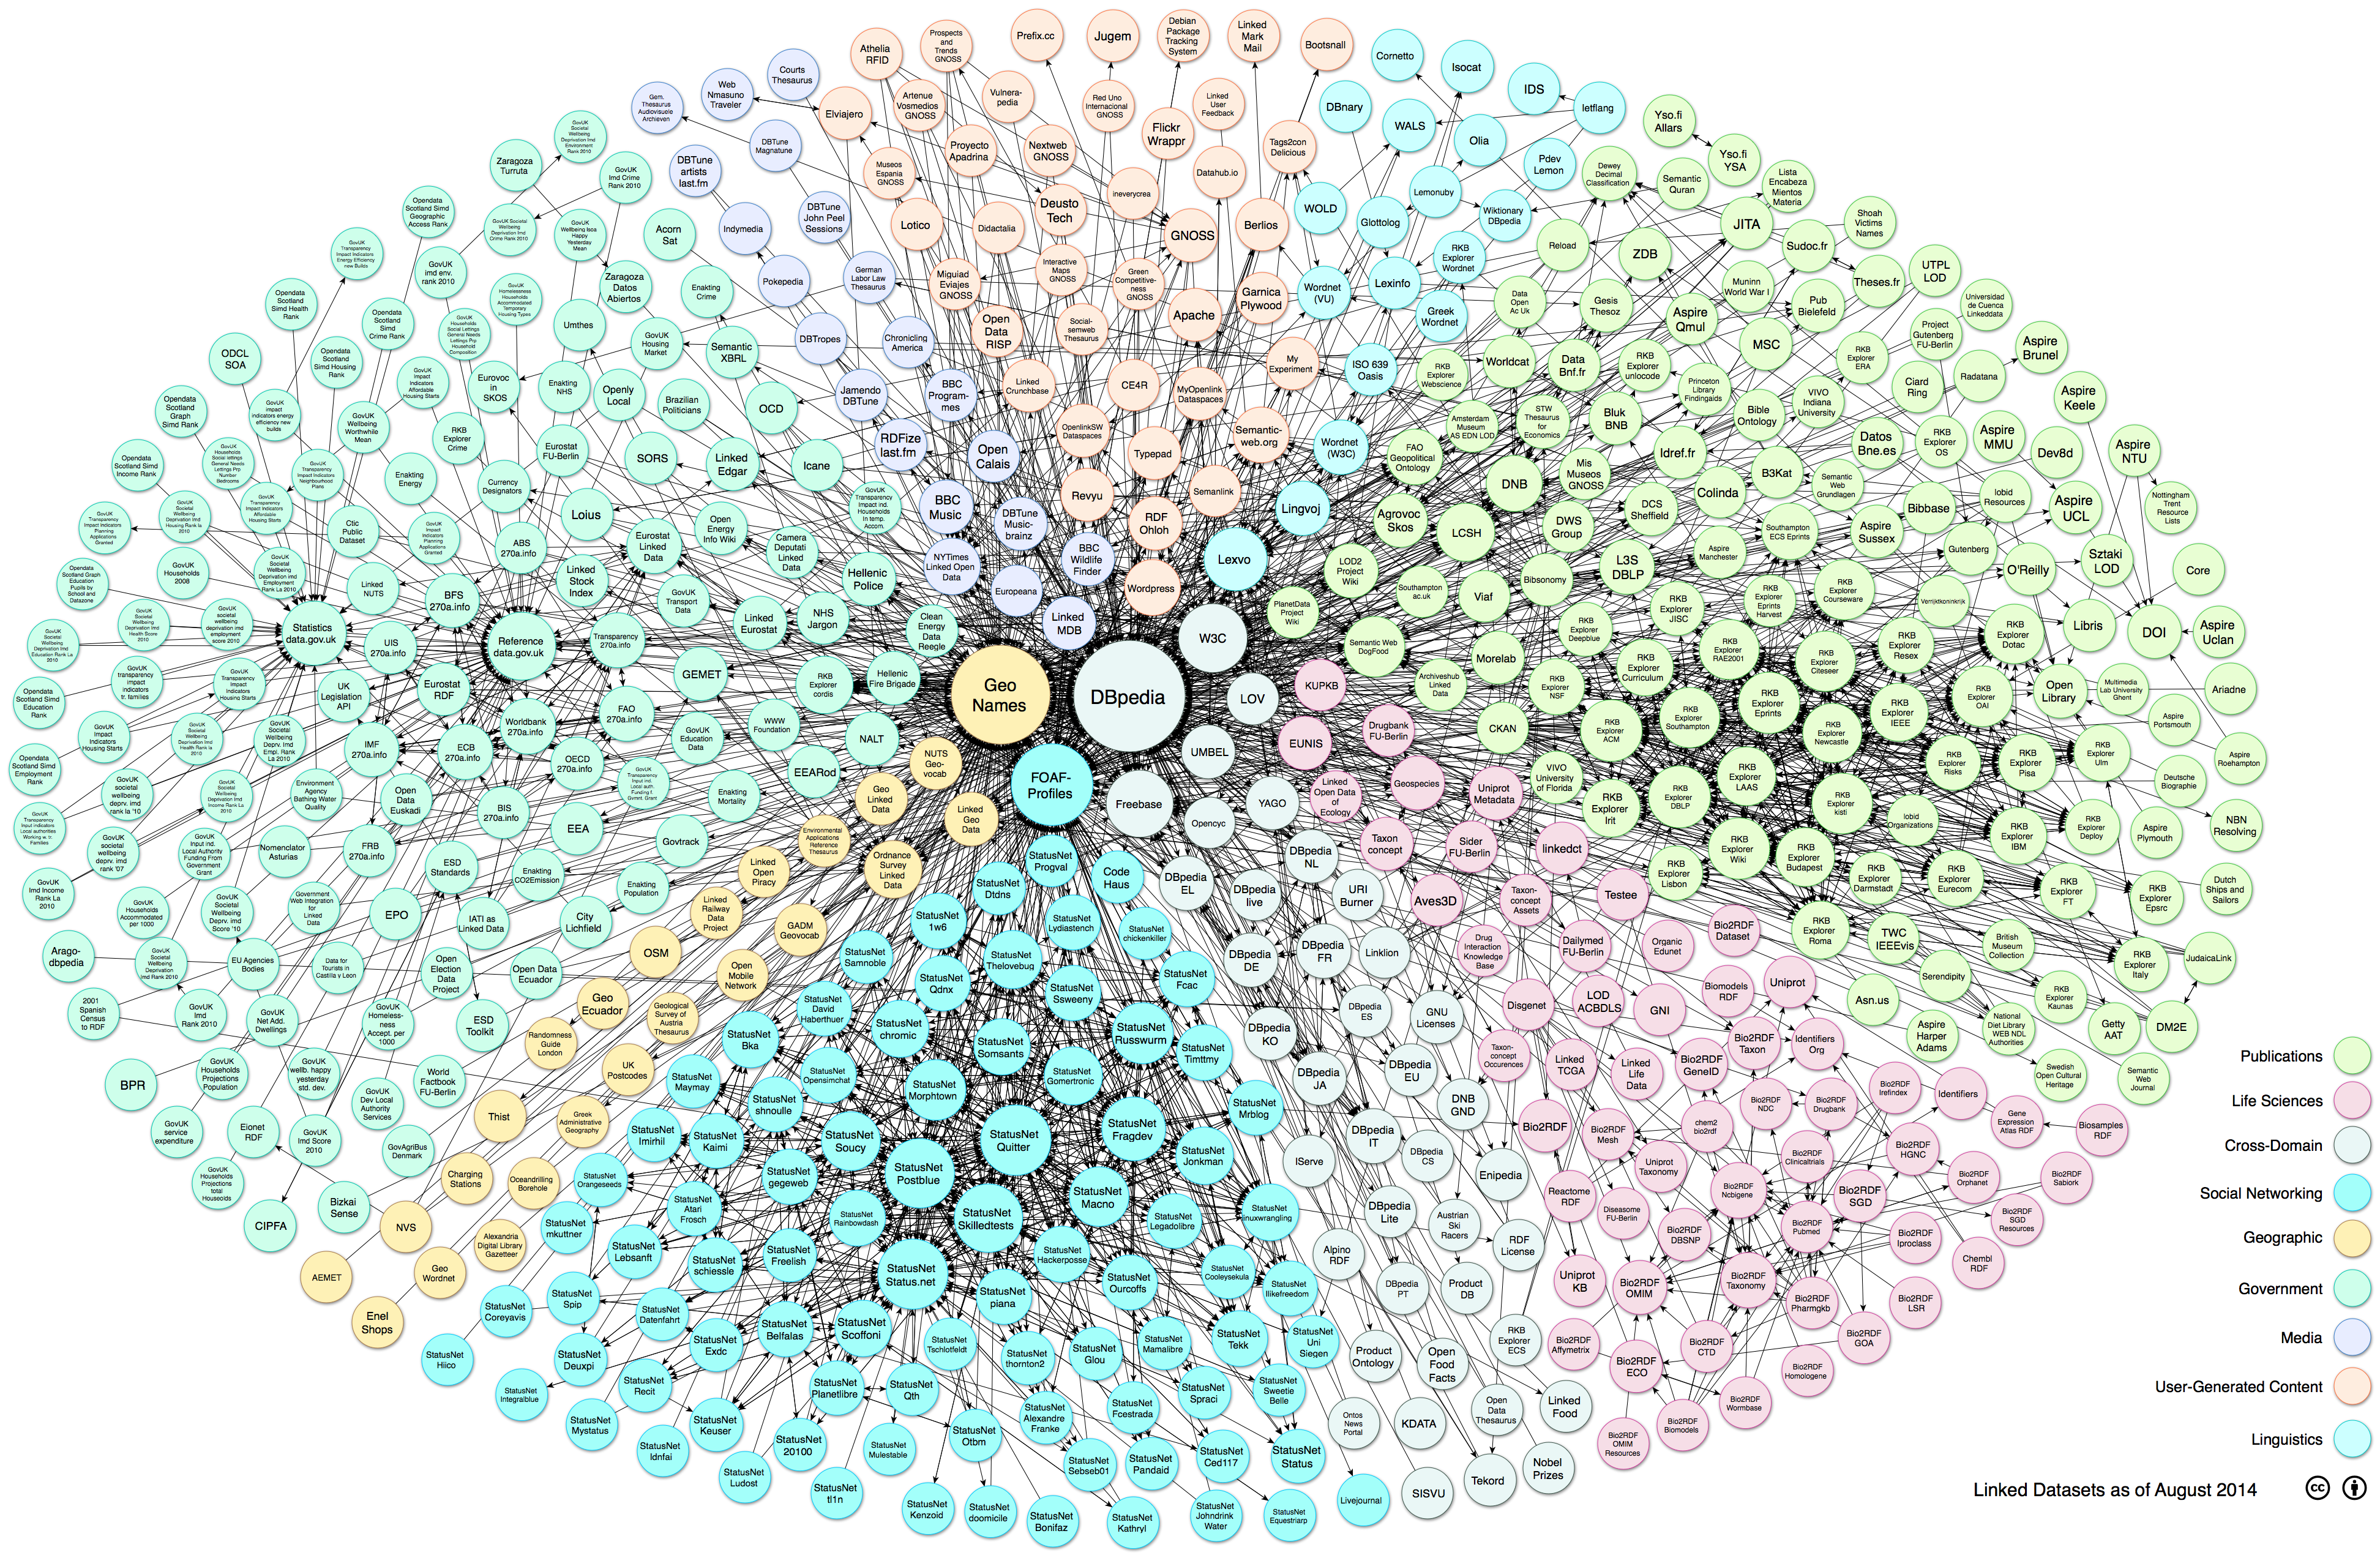
\includegraphics[scale=0.12]{lod-cloud_colored2014.png}
	\end{center}
	\legend{Fonte: \citeonline{grafo}}
\end{figure}

Logo, com o intuito de incentivar principalmente a abertura de dados governamentais, o \citeonline{berners2006linked} 
desenvolveu um sistema de classificação por estrelas, onde apenas dados abertos que obtenham cinco estrelas podem ser 
considerados \emph{Linked Open Data}. O sistema classifica da seguinte maneira:
Uma estrela: Disponibilizar os dados em qualquer formato na \emph{web}, utilizando uma licença aberta;
Duas estrelas: Atender aos requisitos anteriores, e disponibilizar os dados de maneira estruturada para que possam ser legíveis 
por máquinas;
Três estrelas: Atender aos requisitos de todas as classificações anteriores, além de não publicar os dados em nenhum formato 
proprietário;
Quatro estrelas: Atender aos requisitos de todas as classificações anteriores e utilizar padrões abertos da W3C (RDF e SPARQL)
para identificadores, de modo que pessoas possam apontar para os dados publicados;
Cinco estrelas: Atender aos requisitos de todas as classificações anteriores e vincular o dados publicados com de outras 
pessoas para criar um contexto.

Muitos governos já disponibilizam seus dados a partir dos princípios anteriormente apresentados, como Estados Unidos,
Reino Unido, Austrália e Nova Zelândia, \cite{agunegreg}. Apesar da recente existência de dados abertos governamentais,
estes governos já adotam essa teoria como política pública de promoção da transparência. Segundo \citeonline{vaz2011dados}, o Brasil ainda não disponibiliza os
seus dados integralmente utilizando os formatos abertos.

Em 2011, o Brasil tornou-se o 89º país a contar com uma lei geral de acesso a informação pública, a Lei 12.527. De acordo com 
a Lei de Acesso à Informação, é dever dos órgãos e entidades públicas promover, independentemente de requerimentos, a divulgação
em local de fácil acesso, no âmbito de suas competências, de informações de interesse coletivo. Segundo \citeonline{pedroso2013lei}, uma publicação mínima deve ser
efetuada de maneira proativa por órgãos e entidades públicas, denominada transparência ativa.

Segundo \citeonline{brasillei}, não há definição de órgão supervisor independente e exclusivamente voltado para monitorar
e efetivar a lei no Brasil. Apesar da Controladoria Geral da União ser a responsável por implementá-la no âmbito do Executivo
Federal, ela aplica-se a todos os Poderes da República e aos níveis de governo. Por exemplo, embora Judiciário e Legislativo
também estejam cobertos pela lei há poucos relatos sobre sua implementação nesses espaços. Logo, ressalta-se que a ausência de
um órgão responsável tornou-se uma das mais frequentes críticas à Lei de Acesso brasileira.

Apesar disso, tem-se alguns casos de sucesso utilizando dados governamentais abertos no Brasil. Um exemplo é o Radar Parlamentar
, que é um aplicativo que ilustra as semelhanças entre partidos políticos com base na análise matemática dos 
dados de votações que ocorrem na casa legislativa. As semelhanças são apresentadas em um gráfico bidimensional, em que círculos 
representam partidos ou parlamentares, e a distância entre esses círculos representa o quão parecido os mesmos votam. A 
\autoref{radarparlamentar} exibe um gráfico da Câmara dos Deputados gerado pelo aplicativo e a semelhança de votações entre os
partidos. Outros aplicativos podem ser encontrados no Portal Brasileiro de Dados Abertos.

\begin{figure}[htb]
	\caption{\label{radarparlamentar}Gráfico de um biênio da Câmara dos Deputados}
	\begin{center}
	    \includegraphics[scale=0.5]{radarparlamentar.png}
	\end{center}
	\legend{Fonte: Radar Parlamentar}
\end{figure}

\chapter{Conjunto de dados da Câmara dos Deputados} 
A Câmara dos Deputados tem realizado diversas iniciativas para a regulamentação da lei de acesso a informação no órgão. 
Uma delas é o Laboratório Hacker da Câmara dos Deputados, que foi criado pela Resolução nº 49 de 2013, publicada no D.O.U. 
de 18/12/2013, com o objetivo de promover ações colaborativas visando o aprimoramento da transparência legislativa e da 
participação popular. Como definido pela própria Resolução, o Laboratório conta com espaço físico de acesso e uso livres 
para qualquer cidadão, especialmente programadores e desenvolvedores de softwares preferencialmente livres, parlamentares e 
servidores públicos, onde poderão utilizar dados públicos de forma colaborativa para ações de cidadania, \cite{wsproposicoes}.

Para o desenvolvimento do portal foi utilizado o serviço de Dados Abertos da Câmara dos Deputados, que contém uma coleção de 
funcionalidades permitindo o acesso direto aos dados produzidos na Câmara dos Deputados. O conjunto de dados do Legislativo contém dados sobre deputados, órgãos legislativos, proposições, sessões plenárias e reuniões 
de comissões. Tais informações são disponibilizadas através de \emph{web services} ou dados brutos. 
\emph{Web services} são componentes de aplicação utilizados para integrar serviços baseados na \emph{web}, utilizando protocolos 
abertos como XML, SOAP, WSDL, UDDI, entre outros. Para este projeto utilizou-se o SOAP. 

Para \citeonline{soapbook} SOAP é um mecanismo de intercâmbio de mensagens que é endossado por grandes empresas de aplicativos
distribuídos, e divide-se em três partes: (1) Definição de uma representação XML para a intercâmbio das mensagens; (2) Um 
conjunto de convenções para expressar instâncias de tipos de dados definidos pelo aplicativo e (3) Definição de uma 
representação XML para o RPC. O elemento máximo de uma mensagem SOAP é o envelope, que contém um corpo com parâmetros de uma 
chamada e um cabeçalho opcional. O SOAP gerencia a transmissão de status e semântica das chamadas por meio de convenções no 
corpo da própria mensagem e o protocolo com o qual se comunica.

Os \emph{web services} são dividos em:

\begin{itemize}
  \item Deputados: Disponibiliza serviços de acesso aos dados de deputados federais;
  \item Orgaos: Disponibiliza serviços de acesso aos dados dos órgãos legislativos da Câmara dos Deputados;
  \item Proposicoes: Disponibiliza serviços de acesso aos dados das proposições que tramitaram ou que estão em tramitação na Câmara dos Deputados;
  \item SessoesReunioes: Disponibiliza serviços de acesso aos dados das sessões plenárias e das reuniões de comissões realizadas na Câmara dos Deputados.
\end{itemize}

Os dados brutos contém subconjuntos de determinado assunto específico, disponibilizados em CSV ou JSON. Contém os tipos de 
proposição e subconjuntos dos principais tipos de proposição.

Ambos meios de disponibilização permitem o acesso direto aos dados legislativos produzidos, entretanto há variações. 
Através do \emph{web service} Proposicoes é possível encontrar informações de proposições que tramitaram ou estão em tramitação
na Câmara dos Deputados, entretanto é necessário enviar parte do nome do autor para a busca das proposições ou outros parâmetros
como ano e tipo de proposição. Tal obrigatoriedade permite uma busca limitada e a geração de múltiplas pesquisas para mapear
todas as proposições. Os dados brutos contém todas as principais proposições de determinado período, entretanto há mais tipos 
de proposição apreciados pela Câmara, tais como: emendas, pareceres, indicações, etc. Os tipos de proposição considerados
principais, visto que originam as normas descritas no art. 59 da Constituição Federal, são: Propostas de Emenda à Constituição
(PEC), Projetos de Lei Complementar (PLP), Projetos de Lei Ordinária (PL), Projetos de Decreto Legislativo (PDC), Projetos de 
Resolução (PRC) e Medidas Provisórias (MPV). 

Neste contexto, foi necessária uma análise da abrangência de cada meio de disponibilização objetivando um resultado de conjunto
de dados realístico, transparente e funcional para o portal. Durante a análise, foi constatado que os principais tipos de 
proposições são insuficientes para resultar em uma análise estatística real de proposições que tramitam na Câmara dos Deputados.
Também não foi encontrada uma descrição da proposição ao analisar alguns subconjuntos dos dados brutos. Sendo assim, a
utilização dos \emph{web services} disponibilizados mostrou-se mais satisfatória que demais meios.

Entre os \emph{web services} disponibilizados pela Câmara dos Deputados, o 'Proposicoes' foi escolhido para o projeto por
conter mais informações relacionadas às proposições que tramitam ou tramitaram na Câmara dos Deputados. A \autoref{figurafluxoproposicao} 
exibe o fluxo simplificado do processo legislativo na Câmara dos Deputados.
\begin{figure}[htb]
	\caption{\label{figurafluxoproposicao}Fluxo do Processo Legislativo na Câmara dos Deputados}
	\begin{center}
	    \includegraphics[scale=0.9]{fluxo.jpg}
	\end{center}
	\legend{Fonte:\citeonline{wsproposicoes}}
\end{figure}
O processo legislativo é definido pela Constituição Federal e está especificado nos Regimentos Internos do Senado e da Câmara e no 
Regimento Comum do Congresso Nacional e compreende a elaboração de emendas à constituição, leis complementares, leis 
ordinárias, leis delegadas, medidas provisórias, decretos legislativos e resoluções.
De acordo com a \citeonline{wsproposicoes} o \emph{web service} possui vários métodos, os quais são:
\begin{itemize}
  \item ListarProposicoes: Retorna a lista de proposições que satisfaçam os critérios estabelecidos;
  \item ListarSiglasTipoProposicao: Retorna a lista de siglas de proposições;
  \item ListarSituacoesProposicao: Retorna a lista de situações para proposições;
  \item ListarTiposAutores: Retorna a lista de tipos de autores das proposições;
  \item ObterProposicao: Retorna os dados de uma determinada proposição a partir do tipo, número e ano;
  \item ObterProposicaoPorID: Retorna os dados de uma determinada proposição a partir do seu ID;
  \item ObterVotacaoProposicao: Retorna os votos dos deputados a uma determinada proposição em votações ocorridas no Plenário da Câmara dos Deputados;
  \item ListarProposicoesVotadasEmPlenario: Retorna todas as proposições votadas em plenário num determinado período;
  \item ListarProposicoesTramitadasNoPeriodo: Retorna uma lista de proposições movimentadas em determinado período.
\end{itemize}

O método 'ListarProposicoes' retorna a lista de proposições que satisfaçam os critérios estabelecidos. A \autoref{tabela-listarproposicoes}
apresenta os parâmetros recebidos pelo método, assim como seu valor e descrição do campo.

\begin{table}[htb]
\IBGEtab{%
  \caption{Lista de parâmetros do método 'ListarProposicoes'}%
  \label{tabela-listarproposicoes}
}{%
  \begin{tabular}{p{4cm}p{4.0cm}p{7.25cm}}
  \toprule
   Nome & Valor & Descrição \\
  \midrule \midrule
   Sigla & String(Obrigatório se ParteNomeAutor não for preenchido) & Sigla do tipo de proposição \\
  \midrule 
   Número & Int(Opcional) & Número da proposição \\
  \midrule 
  Ano &  Int(Obrigatório se ParteNomeAutor não for preenchido) & Ano da proposição \\
  \midrule 
  datApresentacaoIni &  Date(Opcional) & Menor data desejada para a data de apresentação da proposição.

Formato: DD/MM/AAAA \\
  \midrule 
  datApresentacaoFim &  Date(Opcional) & Maior data desejada para a data de apresentação da proposição 

Formato: DD/MM/AAAA \\
  \midrule 
  IdTipoAutor &  Int(Optional) & Identificador do tipo de órgão autor da proposição, como obtido na chamada ao ListarTiposOrgao \\
  \midrule 
  ParteNomeAutor & String(Optional) & Parte do nome do autor(5 ou + caracteres) da proposição.  \\
  \midrule 
  SiglaPartidoAutor & String(Optional) & Sigla do partido do autor da proposição \\
  \midrule 
  SiglaUfAutor & String(Optional) & UF de representação do autor da proposição \\
  \midrule 
  GeneroAutor & String(Optional) & Gênero do autor<BR>M - Masculino; F - Feminino; Default - Todos \\
  \midrule 
  IdSituacaoProposicao & Int(Opcional) & ID da situação da proposição \\
  \midrule 
  IdOrgaoSituacaoProposicao & Int(Opcional) & ID do órgão de referência da situação da proposição \\
  \midrule 
  EmTramitacao & Int(Opcional) & Indicador da situação de tramitação da proposição<BR>1 - Em Tramitação no Congresso; 2- Tramitação Encerrada no Congresso; Default - Todas \\
  \bottomrule
\end{tabular}%
}{%
  \fonte{\citeonline{wsproposicoes}}%
  
  }
\end{table}

A \autoref{tabela-returnlistarproposicoes} apresenta os dados do retorno do método 'ListarProposicoes', contendo uma lista das proposições que satisfazem os critérios estabelecidos.

O método 'ListarSiglasTipoProposicao' retorna a lista de siglas de proposições, e não possui parâmetros de entrada. A \autoref{tabela-listarsiglasproposicao} apresenta os itens da lista das siglas dos tipos de proposição.

\begin{table}[htb]
\IBGEtab{%
  \caption{Lista de retorno do método 'ListarSiglasTipoProposicao'}%
  \label{tabela-listarsiglasproposicao}
}{%
  \begin{tabular}{p{4cm}p{4.0cm}p{7.25cm}}
  \toprule
   Nome & Valor & Descrição \\
  \midrule \midrule
   Sigla & String & Sigla do tipo da proposição (espécie da proposição) \\
  \midrule
   Descricao & String & Descrição do tipo da proposição (espécie da proposição) \\
  \midrule 
   Ativa & String & Indica se é uma sigla de proposição (espécie da proposição) ativa (1= Ativa; 2=Inativa) \\
  \midrule 
   Genero & String & Indicador do gênero da sigla da proposição (espécie da proposição) \\
  \bottomrule
\end{tabular}%
}{%
  \fonte{\citeonline{wsproposicoes}}%
  
  }
\end{table}

O método 'ListarSituacoesProposicao' retorna a lista de situações para proposições, e
não possui parâmetros de entrada. A \autoref{tabela-situacaoproposicoes} apresenta os itens da lista dos tipos de situação das proposições.

\begin{table}[htb]
\IBGEtab{%
  \caption{Lista de retorno do método 'ListarSituacoesProposicao'}%
  \label{tabela-situacaoproposicoes}
}{%
  \begin{tabular}{p{4cm}p{4.0cm}p{7.25cm}}
  \toprule
   Nome & Valor & Descrição \\
  \midrule \midrule
   ID & Int & ID da situação da proposição \\
  \midrule
   Descricao & String & Descrição da situação da proposição \\
  \midrule
   Ativa & String & Indica se é uma situação ativa (1= Ativa; 0=Inativa) \\
  \bottomrule
\end{tabular}%
}{%
  \fonte{\citeonline{wsproposicoes}}%
  
  }
\end{table}

\begin{table}[htb]
\IBGEtab{%
  \caption{Lista de retorno do método 'ListarProposicoes'}%
  \label{tabela-returnlistarproposicoes}
}{%
  \begin{tabular}{p{4cm}p{4.0cm}p{7.25cm}}
  \toprule
   Nome & Valor & Descrição \\
  \midrule \midrule
   Id & Int & ID da proposição \\
  \midrule
   Nome & String & Nome da proposição \\
  \midrule
   TipoProposicao & TipoProposicao & Dados do tipo da proposição \\
  \midrule
   Numero & Int & Número da proposição \\
  \midrule
   Ano & Int & Ano de apresentação da proposição \\
  \midrule
   OrgaoNumerador & OrgaoNumerador & Orgão onde a proposição foi numerada \\
  \midrule
   DataApresentacao & Date & Data de apresentação da proposição \\
  \midrule
   Ementa & String & Ementa da proposição \\
  \midrule
   ExplicacaoEmenta & String & Explicação da ementa da proposição \\
  \midrule
   Regime & Regime & Regime de tramitação da Proposição (ex: tramitação ordinária, urgência, etc) \\
  \midrule
   Apreciacao & Apreciacao & Forma de apreciação da proposição na Câmara dos Deputados (conclusiva das comissões ou de apreciação do Plenário) \\
  \midrule
   QtdeAutores & Int & Quantidade de autores que subscreveram a proposição \\
  \midrule
   Autor1 & Autor & Primeiro autor da proposição \\
  \midrule
   UltimoDespacho & UltimoDespacho & Último despacho proferido para a proposição \\
  \midrule
   Situacao & Situacao & Situação da proposição na Câmara dos Deputados\\
  \midrule
   ProposicaoPrincipal & ProposicaoPrincipal & Proposição a qual a proposição de referência está associada (apensada ou anexada) \\
  \bottomrule
\end{tabular}%
}{%
  \fonte{\citeonline{wsproposicoes}}%
  
  }
\end{table}

O método 'ListarTiposAutores' retorna a lista de tipos de autores das proposições,
e não possui parâmetros de entrada. A \autoref{tabela-tipoautores} apresenta os itens da lista dos tipos de autor das proposições.

\begin{table}[htb]
\IBGEtab{%
  \caption{Lista de retorno do método 'ListarTiposAutores'}%
  \label{tabela-tipoautores}
}{%
  \begin{tabular}{p{4cm}p{4.0cm}p{7.25cm}}
  \toprule
   Nome & Valor & Descrição \\
  \midrule \midrule
   ID & Strig & ID do tipo de autor \\
  \midrule
   Descricao & String & Descrição do tipo de autor \\
  \bottomrule
\end{tabular}%
}{%
  \fonte{\citeonline{wsproposicoes}}%
  
  }
\end{table}

O método ’ObterProposicao’ retorna os dados de uma determinada proposição a partir do tipo, número e ano. A \autoref{tabela-obterproposicao} apresenta os parâmetros recebidos pelo método, assim
como seu valor e descrição do campo.

\begin{table}[htb]
\IBGEtab{%
  \caption{Parâmetros do método 'ObterProposicao'}%
  \label{tabela-obterproposicao}
}{%
  \begin{tabular}{p{4cm}p{4.0cm}p{7.25cm}}
  \toprule
   Nome & Valor & Descrição \\
  \midrule \midrule
   Tipo & String (Obrigatorio) & Sigla do tipo de proposição \\
  \midrule
   Numero & Int (Obrigatorio) & Numero da proposição \\
  \midrule
   Ano & Int (Obrigatorio) & Ano da proposição \\
  \bottomrule
\end{tabular}%
}{%
  \fonte{\citeonline{wsproposicoes}}%
  
  }
\end{table}

A \autoref{tabela-returnobterproposicao} apresenta os dados do retorno do método ’ListarProposicoes’, contendo os dados da proposição que satisfaça os critérios estabelecidos.


\begin{table}[htb]
\IBGEtab{%
  \caption{Retorno do método 'ObterProposicao'}%
  \label{tabela-returnobterproposicao}
}{%
  \begin{tabular}{p{4cm}p{4.0cm}p{7.25cm}}
  \toprule
   Nome & Valor & Descrição \\
  \midrule \midrule
   Tipo & String & Tipo da proposição \\
  \midrule
   Numero & Int & Numero da proposição \\
  \midrule
   Ano & Int & Ano de apresentação da proposição \\
  \midrule
   IdProposicao & Int & ID da proposição \\
  \midrule
   Ementa & String & Ementa da proposição \\
  \midrule
   ExplicacaoEmenta & String & Explicação da ementa da proposição \\
  \midrule
   Autor & String & Nome do autor da proposição \\
  \midrule
   DataApresentacao & Date & Data em que a propsoição foi apresentada na Câmara dos Deputados \\
  \midrule
   RegimeTramitacao & String & Regime de tramitação da Proposição (ex: tramitação ordinária, urgência, etc) \\
  \midrule
   UltimoDespacho & String & Último despacho proferido para a proposição \\
  \midrule
   Apreciacao & String & Forma de apreciação da proposição na Câmara dos Deputados (conclusiva das comissões ou de apreciação do Plenário) \\
  \midrule
   Indexacao & String & Indexação (palavras-chave) associada à proposição \\
  \midrule
   Situacao & String & Descrição da situação da proposição na Câmara dos Deputados \\
  \midrule
   LinkInteiroTeor & String & URL contendo o link para o inteiro teor da proposição \\
  \midrule
   apensadas & List<proposicao> & Proposições com assuntos semelhantes \\
  \bottomrule
\end{tabular}%
}{%
  \fonte{\citeonline{wsproposicoes}}%
  
  }
\end{table}

O método ’ObterProposicaoPorID’ retorna os dados de uma determinada proposição a partir do seu ID. A \autoref{tabela-obterproposicaoporid} apresenta os parâmetros recebidos pelo método, assim
como seu valor e descrição do campo.

\begin{table}[htb]
\IBGEtab{%
  \caption{Parâmetros do método 'ObterProposicaoPorID'}%
  \label{tabela-obterproposicaoporid}
}{%
  \begin{tabular}{p{4cm}p{4.0cm}p{7.25cm}}
  \toprule
   Nome & Valor & Descrição \\
  \midrule \midrule
   IdProp & Int (Obrigatorio) & ID da proposição desejada \\
  \bottomrule
\end{tabular}%
}{%
  \fonte{\citeonline{wsproposicoes}}%
  
  }
\end{table}

A \autoref{tabela-returnobterproposicaoporid} apresenta os dados do retorno do método ’ObterProposicaoPorID’, contendo os dados da proposição que satisfaça os critérios estabelecidos.


\begin{table}[htb]
\IBGEtab{%
  \caption{Retorno do método 'ObterProposicao'}%
  \label{tabela-returnobterproposicaoporid}
}{%
  \begin{tabular}{p{4cm}p{4.0cm}p{7.25cm}}
  \toprule
   Nome & Valor & Descrição \\
  \midrule \midrule
   Tipo & String & Tipo da proposição \\
  \midrule
   Numero & Int & Numero da proposição \\
  \midrule
   Ano & Int & Ano de apresentação da proposição \\
  \midrule
   IdProposicao & Int & ID da proposição \\
  \midrule
   idProposicaoPrincipal & Int & ID da Proposição Principal quando a proposição pesquisada for acessória \\
  \midrule
   Ementa & String & Ementa da proposição \\
  \midrule
   ExplicacaoEmenta & String & Explicação da ementa da proposição \\
  \midrule
   Autor & String & Nome do autor da proposição \\
  \midrule
   DataApresentacao & Date & Data em que a propsoição foi apresentada na Câmara dos Deputados \\
  \midrule
   RegimeTramitacao & String & Regime de tramitação da Proposição (ex: tramitação ordinária, urgência, etc) \\
  \midrule
   UltimoDespacho & String & Último despacho proferido para a proposição \\
  \midrule
   Apreciacao & String & Forma de apreciação da proposição na Câmara dos Deputados (conclusiva das comissões ou de apreciação do Plenário) \\
  \midrule
   Indexacao & String & Indexação (palavras-chave) associada à proposição \\
  \midrule
   Situacao & String & Descrição da situação da proposição na Câmara dos Deputados \\
  \midrule
   LinkInteiroTeor & String & URL contendo o link para o inteiro teor da proposição \\
  \midrule
   apensadas & List<proposicao> & Proposições com assuntos semelhantes \\
  \bottomrule
\end{tabular}%
}{%
  \fonte{\citeonline{wsproposicoes}}%
  
  }
\end{table}

O método ’ObterVotacaoProposicao’ retorna os votos dos deputados a uma determinada proposição em votações ocorridas no Plenário da Câmara dos Deputados. A \autoref{tabela-obtervotacao} apresenta os parâmetros recebidos pelo método, assim
como seu valor e descrição do campo.

\begin{table}[htb]
\IBGEtab{%
  \caption{Parâmetros do método 'ObterVotacaoProposicao'}%
  \label{tabela-obtervotacao}
}{%
  \begin{tabular}{p{4cm}p{4.0cm}p{7.25cm}}
  \toprule
   Nome & Valor & Descrição \\
  \midrule \midrule
   Tipo & String (Obrigatorio) & Sigla do tipo de proposição \\
  \midrule
   Numero & Int (Obrigatorio) & Numero da proposição \\
  \midrule
   Ano & Int (Obrigatorio) & Ano da proposição \\
  \bottomrule
\end{tabular}%
}{%
  \fonte{\citeonline{wsproposicoes}}%
  
  }
\end{table}

A \autoref{tabela-returnobtervotacao} apresenta os dados do retorno do método ’ObterVotacaoProposicao’, contendo os dados da votação da proposição.

\begin{table}[htb]
\IBGEtab{%
  \caption{Retorno do método 'ObterVotacaoProposicao'}%
  \label{tabela-returnobtervotacao}
}{%
  \begin{tabular}{p{4cm}p{4.0cm}p{7.25cm}}
  \toprule
   Nome & Valor & Descrição \\
  \midrule \midrule
   Sigla & String & Sigla do Tipo da proposicao \\
  \midrule
   Numero & Int & Numero da proposição \\
  \midrule
   Ano & Int & Ano de apresentação da proposição \\
  \midrule
   Votacoes & List<Votacao> & Lista das votações nominais em Plenário da proposição \\
  \bottomrule
\end{tabular}%
}{%
  \fonte{\citeonline{wsproposicoes}}%
  
  }
\end{table}

O método 'ListarProposicoesVotadasEmPlenario' retorna a lista de proposições que sofreram votação em plenário em determinado ano. A \autoref{tabela-votadasemplenario} apresenta os parâmetros recebidos pelo método, assim
como seu valor e descrição do campo.

\begin{table}[htb]
\IBGEtab{%
  \caption{Parâmetros do método 'ListarProposicoesVotadasEmPlenario'}%
  \label{tabela-votadasemplenario}
}{%
  \begin{tabular}{p{4cm}p{4.0cm}p{7.25cm}}
  \toprule
   Nome & Valor & Descrição \\
  \midrule \midrule
   Ano & Int (Obrigatorio) & Ano da proposição \\
  \midrule
   Tipo & String(Opcional) & Tipo de proposição \\
  \bottomrule
\end{tabular}%
}{%
  \fonte{\citeonline{wsproposicoes}}%
  
  }
\end{table}

A \autoref{tabela-returnvotadasemplenario} apresenta os itens da lista contendo todas as proposições que satisfazem os critérios estabelecidos.

\begin{table}[htb]
\IBGEtab{%
  \caption{Retorno do método 'ListarProposicoesVotadasEmPlenario'}%
  \label{tabela-returnvotadasemplenario}
}{%
  \begin{tabular}{p{4cm}p{4.0cm}p{7.25cm}}
  \toprule
   Nome & Valor & Descrição \\
  \midrule \midrule
   codProposicao & Int & ID da proposição \\
  \midrule
   nomeProposicao & Sring & Nome da proposição \\
  \bottomrule
\end{tabular}%
}{%
  \fonte{\citeonline{wsproposicoes}}%
  
  }
\end{table}

O método ’listarProposicoesTramitadasNoPeriodo’ retorna a  lista de proposições que tramitaram em determinado período. O período máximo é de 7 dias. A \autoref{tabela-tramitadasperiodo} apresenta os parâmetros recebidos pelo método, assim
como seu valor e descrição do campo.

\begin{table}[htb]
\IBGEtab{%
  \caption{Parâmetros do método 'listarProposicoesTramitadasNoPeriodo'}%
  \label{tabela-tramitadasperiodo}
}{%
  \begin{tabular}{p{4cm}p{4.0cm}p{7.25cm}}
  \toprule
   Nome & Valor & Descrição \\
  \midrule \midrule
   dtInicio & String (Obrigatorio) & Data de início \\
  \midrule
   dtFim & String (Obrigatorio) & Data final \\
  \bottomrule
\end{tabular}%
}{%
  \fonte{\citeonline{wsproposicoes}}%
  
  }
\end{table}

A \autoref{tabela-returntramitadasperiodo} apresenta os itens da lista contendo todas as proposições que satisfazem os critérios estabelecidos.

\begin{table}[htb]
\IBGEtab{%
  \caption{Retorno do método 'listarProposicoesTramitadasNoPeriodo'}%
  \label{tabela-returntramitadasperiodo}
}{%
  \begin{tabular}{p{4cm}p{4.0cm}p{7.25cm}}
  \toprule
   Nome & Valor & Descrição \\
  \midrule \midrule
   codProposicao & String & Código da proposição \\
  \midrule
   tipoProposicao & Sring & Tipo da proposição \\
  \midrule
   Numero & Sring & Número da proposição \\
  \midrule
   Ano & Sring & Ano da proposição \\
  \bottomrule
\end{tabular}%
}{%
  \fonte{\citeonline{wsproposicoes}}%
  
  }
\end{table}

\chapter{O portal} 
O portal, denominado 'Eaicongresso', terá como objetivo principal apresentar de maneira clara e objetiva as proposições que tramitaram ou tramitam na Câmara dos 
Deputados, assim como análises específicas sobre os dados. Todas as ferramentas utilizadas durante o desenvolvimento serão grátis 
e/ou \emph{open source}, e compatíveis com o sistema operacional Linux. Todo o projeto será disponibilizado em repositório público.

Utilizando o \emph{web service} 'Proposicoes', a base de dados da aplicação será atualizada diariamente 
e fornecerá todas as informações necessárias para o portal. A busca de proposições poderá ser efetuada de três maneiras: (1) Pela escolha de determinado tema como saúde, educação, segurança, entre outros;
(2) Por determinado intervalo de datas; (3) Por nível de relevância de acordo com a funcionalidade de votação, ordenando-as de 
maneira crescente ou decrescente. O portal exibirá as proposições que estarão em votação na data do acesso, exibindo o código, 
assunto e descrição sucinta. Outra funcionalidade será a Votação, que permitirá o usuário final votar em determinada proposição, considerando-a relevante ou irrelevante.

O portal também terá oito análises, que serão representadas graficamente: (1) Analisar a quantidade de proposições que entraram e saíram por determinado período; (2) 
Analisar a proporção de cada tema relacionado com o todo de proposições, considerando o período de doze meses; (3) Analisar a proporção de 
cada tipo de proposição relacionado com o número total, considerando o período de doze meses; (4) Analisar quais meses houveram 
mais proposições tramitadas e em qual período o número foi abaixo da média geral de todos os meses, considerando um período de quatro anos; (5)
Analisar a proporção de participação de cada tipo de autor relacionado com o número total de proposições, considerando o período de doze meses; (6)
Analisar o número total de proposições apresentadas no período de oito anos, através de um gráfico de linhas; (7) Analisar quais os cinco temas mais relevantes 
para a população de acordo com a votação geral contabilizada no portal e (8) Analisar o número total de proposições apresentadas durante os últimos três mandatos presidenciais, através de um gráfico de linhas.

Como uma das premissas do projeto são ferramentas open source, gratuitas e compatíveis com o sistema operacional Linux,
buscou-se opções dentro de tais requisitos uma para criar a modelagem do banco de dados do portal. Entre as 
ferramentas pesquisadas destacou-se a MySQL Workbench, provendo dentre outros recursos, desenho e modelagem de banco de dados.
A ferramenta permite visualizar o design, modelagem, gerar e gerenciar bases de dados e criar modelos complexos 
de Entidade Relacionamento.

Esta modelagem inicial, conforme apresentado na \autoref{modelagemeaicongresso}, não abrange as funcionalidades de análise e processamento dos dados contidas no portal. A \autoref{modelagemsimplificada} 
exibe as principais entidades do banco de dados de maneira simplificada.

\begin{figure}[htb]
	\caption{\label{modelagemsimplificada}Entidades da base de dados do portal}
	\begin{center}
	    \includegraphics[scale=0.65]{modeloaicongressosimplificado.png}
	\end{center}
	
\end{figure}

\begin{figure}[htb]
	\caption{\label{modelagemeaicongresso}Modelagem da base de dados do portal}
	\begin{center}
	    \includegraphics[scale=0.65]{modeloaicongresso.png}
	\end{center}
	
\end{figure}

Também foi necessário realizar um mapeamento dos dados entre o \emph{web service} e a aplicação. A \autoref{tabela-deparaaplicacao} 
apresenta o método que será utilizado para obter o dado assim como seu campo, e tabela e coluna de destino. Alguns 
retornos do método são objetos que estão definidos na modelagem do banco de dados do portal, entretanto não foram citados explicitamente
nesta relação para tal não conter informações redundantes.

\begin{table}[htb]
\IBGEtab{%
  \caption{Relação 'De' 'Para' entre o \emph{web service} e o portal}%
  \label{tabela-deparaaplicacao}
}{%
  \begin{tabular}{p{4cm}p{3cm}p{2cm}p{3cm}}
  \toprule
   Método & Campo & Tabela & Coluna \\
  \midrule \midrule
  ListarProposicoes & IdProposicao & Proposição & id \\
  \midrule 
  ListarProposicoes & Nome & Proposição & nome \\  
  \midrule 
  ListarProposicoes & TipoProposicao & Proposição & tipo proposicao \\  
  \midrule 
  ListarProposicoes & Numero & Proposição & numero \\  
  \midrule 
  ListarProposicoes & Ano & Proposição & ano \\  
  \midrule 
  ListarProposicoes & OrgaoNumerador & Proposição & orgao numerador \\ 
  \midrule 
  ListarProposicoes & DataApresentacao & Proposição & data apresentacao \\   
  \midrule 
  ListarProposicoes & Ementa & Proposição & ementa \\  
  \midrule 
  ListarProposicoes & ExplicacaoEmenta & Proposição & explicacao ementa \\  
  \midrule 
  ListarProposicoes & Regime & Proposição & regime \\  
  \midrule 
  ListarProposicoes & Apreciacao & Proposição & apreciacao \\  
  \midrule 
  ListarProposicoes & QtdeAutores & Proposição & qtde autores \\  
  \midrule 
  ListarProposicoes & Autor1 & Proposição & autor principal \\  
  \midrule 
  ListarProposicoes & Situacao & Proposição & situacao \\  
  \midrule 
  ObterProposicao & Indexacao & Proposição e Indexação & Id da proposição e id da indexação \\  
  \midrule 
  ListarSiglasTipoProposicao & Sigla & Tipo Proposição & sigla \\  
  \midrule 
  ListarSiglasTipoProposicao & Descrição & Tipo Proposição & descricao \\ 
  \midrule 
  ListarTiposAutores & Id & Tipo autor & descricao \\
  \midrule 
  ListarTiposAutores & Descrição & Tipo autor & descricao \\ 
  \midrule 
  ListarSituacoesProposicao & id & Situação & id \\ \midrule 
  ListarSituacoesProposicao & Descrição & Situação & descricao \\ \midrule 
  ListarSituacoesProposicao & ativa & Situação & ativa \\    
  \bottomrule
  \end{tabular}%
}{%
  %
  
  }
\end{table}

\chapter{Desenvolvimento do portal}
Esta seção irá descrever todo o processo de desenvolvimento do portal facilitador de acesso a dados governamentais públicos. A linguagem utilizada para implementação 
da aplicação é o Python.

Todos os dados da aplicação como documentação, código fonte, imagens e \emph{scripts} estão disponíveis em 
um repositório remoto através do GitHub, que é um serviço de hospedagem distribuído desenvolvido em linguagem Ruby on Rails para projetos de código aberto que
utilizam o controle de versão Git. O Git é basicamente um sistema de versionamento de arquivos, onde é possível controlar várias alterações em um mesmo arquivo e voltá-lo para versões anteriores, assim como trabalhar em equipe sem maiores 
problemas com a edição de um mesmo projeto.
O repositório criado foi chamado de 'eaicongresso' e está disponível para acesso através do endereço https://github.com/kerollaine/eaicongresso.

\section{O banco de dados}
Algumas regras de negócio foram implementadas dentro da aplicação de banco de dados utilizando procedimentos armazenados, que são conjuntos
de instruções SQL que podem conter parâmetros de entrada e/ou saída e não retornam resultados, ao contrário de funções que 
obrigatoriamente tem um retorno declarado. Para as funções foi utilizado o PL/pgSQL, que é uma linguagem procedural para o banco de 
dados PostgreSQL que pode ser usado para criar funções e \emph{triggers}, adicionar estruturas de controle para a 
linguagem SQL, fazer cálculos complexos, herdar tipos de dados definidos pelos usuários, funções e operadores. A escolha de um sistema 
gerenciador de banco de dados eficiente foi vital para que o processo de importação dos dados para o portal ocorresse com boa performance. 

O sistema gerenciador de banco de dados escolhido foi o PostgreSQL, instalado através do gerenciador de pacotes do sistema operacional denominado Ubuntu 14.04.
O \emph{script} de criação das tabelas da base de dados do portal foi implementado utilizando um editor de arquivos chamado Sublime e os testes foram realizados em um serviço
de execução de \emph{scripts online} chamado SQLFiddle. Outro teste realizado antes de persistir as alterações no banco de dados foi a execução do \emph{script} através utilização das cláusulas \emph{begin} e \emph{rollback}, o qual reverte as alterações ao estado inicial antes da transação. Para 
a aplicação foi criado um usuário para acesso e um banco de dados chamado 'eaicongresso'. 

O projeto é composto por três funções. A função denominada 'importar\_tramitacao' recebe como parâmetros um \emph{id} 
de proposição e uma data, e tem como objetivo inserir os dados obtidos da consulta ao método 'listarProposicoesTramitadasNoPeriodo'
do \emph{web service} na base de dados da aplicação, pois assim será possível importar as proposições. A função 'atualiza\_status\_proposicao' 
busca a proposição cadastrada e altera o campo 'desatualizada' para valor verdadeiro. Assim, sempre
que houver alterações a aplicação saberá quais registros foram alterados e efetuar a correção.

Já a função 'obter\_proposicao' recebe como parâmetros todos os dados para popular as tabelas do item referenciado, buscando sempre
se o valor já existe no banco de dados do portal e caso negativo, inserindo o novo registro. Para que não ocorra inconsistências, 
todos os valores de determinada proposição em tabelas do tipo \emph{many too many} são deletados antes de uma atualização ou nova 
inserção sobre a proposição em questão. Em casos como o tema, foi necessário trabalhar com listas compostas de outras listas para que 
o conteúdo fosse obtido.

\section{Consumindo o \emph{web service}}
Para consumir os dados disponibilizados foram pesquisadas várias bibliotecas em Python para utilizar o SOAP, mas a única disponível
e atualizada recentemente é a PySimpleSOAP. Entretanto ao acessar o \emph{web service} da câmara dos deputados,a mensagem de retorno 'Nossos sistemas automáticos de segurança impediram que a operação fosse concluída.
Isso pode ocorrer quando você copia dados de outros sites e eles vêm com conteúdos não permitidos.' é exibida. A central de atendimento do serviço informou que estão
cientes do problema de instabilidade do serviço e que não tem um prazo final para a resolução do problema. Há várias \emph{issues} cadastradas 
no repositório de dados abertos relatando problemas de indisponibilidade de serviços mas nenhuma solução foi encontrada.

Logo, foi necessário alterar a forma de importar os dados necessários para requisições via protocolo HTTP diretas, utilizando a biblioteca 'requests' do Python onde o resultado é um retorno no formato \emph{string}. Para traduzir
o retorno para XML foi utilizada uma biblioteca chamada ElementTree. Assim, é possível percorrer o arquivo identificando as tags e 
separando as variáveis para o processamento dos dados através da aplicação do portal.

\section{A rotina de importação}
Durante o desenvolvimento da rotina de importação dos dados disponibilizados para a aplicação foi verificada 
uma diferença entre a documentação encontrada e os dados recebidos. Como exemplo pode-se citar o 'OrgaoNumerador' e 'Orgao' que são a mesma
tabela e informações. Logo, a tabela 'Orgao' inicialmente prevista no projeto do portal foi excluída, mantendo apenas a outra. A 
coluna 'idOrgao' da tabela 'situacao' também foi excluída pois não há sentido dentro do contexto da tabela.

Outros problemas foram encontrados durante a importação como extrações sem código identificador ou registros duplicados, que seriam
utilizados como chave primária dentro de seu escopo. Problemas como estes tornam impossível a utilização
de vários métodos disponibilizados, sendo necessário extrair a maioria dos dados do método 'ListarProposicoes' para popular 
as tabelas da aplicação em desenvolvimento.

Para obter uma amostra da quantidade de proposições que serão tratadas por ano, foi implementado um contador de proposições. 
Para isso, inicialmente fez-se a requisição para o método 'ListarSiglasTipoProposição' onde será formado um conjunto de siglas
para acessar o 'ListarProposicoes', onde os parâmetros mínimos de sigla e ano são obrigatórios.

Após, como teste, foi realizada a requisição para o método 'ListarProposicoes' enviando as siglas para o ano de 2015 e contando
todas as proposições encontradas no retorno XML. Em 2014 foram encontradas 14468 proposições. Analisando os dados adquiridos durante a 
amostra observou-se que nem todas as informações necessárias para o portal estão no retorno do método 'ListarProposicoes' e que para 
isso seria necessário chamar o método 'ObterProposicaoPorID', pois contém campos como o 'indexacao' e o 'tema' que são 
extremamente importantes para várias análises que o portal fará sobre os dados. Como premissa, duas chamadas custa mais 
que uma chamada ao serviço externo através da internet. 

Outra divergência encontrada foi que apesar da existência de um método para listar o tipo de autor em nenhum 
resultado de outros métodos utilizados este campo é vinculado, sendo que para relacionar este tipo de autor à 
algum autor seja necessário utilizar outro \emph{web service} específico denominado Deputados, onde uma busca pelo \emph{id} 
seria realizada, saindo do escopo de proposição e dificultando o processo de importação de dados para o portal, tornando-o 
assim inviável. Outra ocorrência evidenciada apenas após os testes foi o 'ideCadastro' do autor da proposição, 
que aparece como nulo quando a autoria é relacionada à determinada comissão. Logo, este campo não pôde ser utilizado pela aplicação.

Durante esta etapa do desenvolvimento houve muita dificuldade para entender alguns registros, como por exemplo
o 'idOrgao' retornado em um conjunto de situações. Em nenhum diretório foi encontrada documentação detalhada sobre a 
relação de cada dado com o conjunto extraído, sendo necessário tempo extra para implementação e execução de testes para entender 
o cenário a ser trabalhado, contexto e escopo das informações.

Sendo assim, muitas tabelas mudaram a sua representação na aplicação apenas para colunas do tipo \emph{string} da proposição
já que terão que ser alteradas sempre que houver uma nova tramitação e não tem-se um \emph{web service} para atualizar a tabela como um 
todo diretamente. O processo de importação dos dados é demorado e pesado. Para o auto incremento dos identificadores dos registros
no banco de dados foi necessário alterar todas as colunas denominadas 'id' 
de tipo \emph{integer} para \emph{serial}. A maioria dos procedimentos inseridos em funções do banco de dados consiste em comparar determinado dado em texto, tratá-lo
para tirar os espaços e vírgulas ou ponto e vírgula, verificar se o registro já existe no banco de dados e retornar o \emph{id} ou caso negativo 
vincular um novo \emph{id} e fazer uma nova inserção.

Este tratamento é realizado através da utilização de expressões regulares, que foi muito utilizada no projeto e consiste em uma 
notação para representar padrões em \emph{strings}, ou seja, um conjunto de símbolos que formam uma expressão que será interpretada
como uma regra para, por exemplo, filtrar determinada frase e retirar vírgulas e pontos.

A rotina de importação consiste em obter as proposições que foram marcadas como desatualizadas durante a importação de todas as 
tramitações no período selecionado, e depois iniciar uma rotina para fazer várias requisições ao servidor da câmara dos deputados 
para obter detalhes de cada proposição, buscando por \emph{id}. Como o resultado dos métodos diferem entre si, este foi o único 
meio de obter informações para indexar as proposições posteriormente, como por exemplo o tema.

Entretanto, no início dos testes foi identificada uma longa demora entre a resposta de uma requisição e outra com tempo superior à 
5 segundos em alguns períodos, evidenciando um gargalo do lado do servidor do \emph{web service} e tornando inviável processar mais 
de 117000 requisições com esta performance. 

Para resolver este problema utilizou-se o conceito de \emph{threads}. \emph{Threads} são processos leves que contém contador de programa, conjunto
de registradores e uma pilha de execução. São estruturas de execução pertencentes a um processo e assim compartilham os segmentos de
código e dados e os recursos alocados ao sistema operacional pelo processo. \emph{Threads} podem ser executadas paralelamente dentro do
contexto da aplicação, cada uma executando o seu processo de maneira independente. São definidos quatro estados de execução para 
uma {\emph{thread}, que são eles: (1) novo, quando uma área de memória é alocada para ela; (2) executável, quando for escalonada para
execução; (3) bloqueado, quando for desativada com algum método como o \emph{sleep} e (4) encerrado, quando a execução for finalizada.

Para cada execução do laço de repetição criado na rotina de importação, foram criadas sete \emph{threads}, cada uma buscando dez
registros para obter proposição. Após o \emph{start}, foi dado a cada processo um \emph{sleep} de 1 segundo. Após, todas as
\emph{threads} foram inseridas em uma lista e agrupadas com o processo principal, através do comando \emph{join}.

Ainda assim foi necessário limitar o número de \emph{threads} para cada requisição, pois com um valor superior o servidor 
retornou mensagens notificando que o número máximo de requisições foi excedido. Também foi necessário colocar todas as threads 
para dormir, criando um atraso, com a finalidade de diminuir a incidência do mesmo erro ao invés do retorno esperado. 

Utilizando esta solução foram importadas em média 50 proposições por minuto. Como eram 117756 proposições iniciais, foram necessárias 
aproximadamente 39 horas para fazer a importação inicial. Foram importadas todas as proposições que foram tramitadas de 2010 até 2015. Para 
cada transação um \emph{commit} foi efetuado, que significa finalizá-la e persistir as alterações no sistema gerenciador de banco de dados.
Com o objetivo de identificar todas as falhas durante a importação, todas as etapas da execução foram registradas em um arquivo de \emph{log}, denominado
'rotina\_importacao.log'. Para isso, foi utilizada a biblioteca \emph{'logging'} do Python.

\section{Processamento de Linguagem Natural e \emph{stop words}}
Entende-se por linguagem natural as linguagens utilizadas para comunicações no cotidiano, por seres humanos. O processamento de
linguagens naturais, também conhecido como linguística computacional engloba qualquer tipo de manipulação computacional de 
linguagens naturais. Tecnologias baseadas neste conceito estão se tornando cada vez mais frequentes, como por exemplo telefones
oferecerem suporte a predição de texto e reconhecimento de escrita ou motores de pesquisa permitirem acessar informações em textos
não estruturados. \cite{nltk}

Neste projeto foi utilizado o framework \emph{Natural Language Toolkit} (NLTK), que contém um conjunto de bibliotecas e programas 
para o processamento de linguagens naturais, desenvolvido em Python e destina-se a apoiar a pesquisa e ensino de linguística 
computacional ou áreas afins, como ciência cognitiva, inteligência artificial, recuperação de informações ou aprendizagem de máquina.

Os módulos do NLTK utilizados neste projeto foram o 'nltk.corpus', com \emph{interfaces} padrão para córpora e léxicos e 'nltk.tokenize'
para o processamento de \emph{strings}.

Para o processar as ementas e temas e indexá-las também foram descartadas as palavras de um conjunto denominado \emph{stop words},
onde as palavras contidas são consideradas irrelevantes para o conjunto de resultados. O conjunto utilizado veio do módulo 
'nltk.corpus', importação denominada 'stopwords'.


\section{A rotina de indexação}
Para possibilitar a pesquisa através do tema ou conteúdo de determinada proposição é necessário processar as informações de forma que a 
recuperação dos dados seja realizada de maneira rápida. Inicialmente foi identificado um campo que continha palavras-chave relacionadas a cada item, denominado 'indexacao'. Mas
após a importação dos dados foi constatado que muitas proposições continham este campo com o valor nulo. Logo, foi necessário alterar os campos a serem indexados 
pelo portal, e foram selecionados os campos 'tema' e 'ementa' para este propósito.

Outro requisito é ordenar os resultados por quantidade de correspondências
encontradas entre os caracteres pesquisados e os dados contidos no banco de dados. Para isso, foi necessário indexar tais dados utilizando uma estrutura
de dados chamada lista invertida, onde uma lista de chaves primárias é associada à uma outra lista com chaves secundárias, conforme 
exemplificado na \autoref{listainvertida}. Esta
estrutura de dados permite uma ótima indexação e é utilizada em motores de busca como o Google, ou sistemas de gerenciamento de 
banco de dados. A desvantagem é a maior dificuldade em atualizar e inserir novas informações.

\begin{figure}[htb]
	\caption{\label{listainvertida}Exemplo de funcionamento da lista invertida}
	\begin{center}
	    \includegraphics[scale=0.65]{listainv.jpg}
	\end{center}
	\legend{Fonte:\citeonline{devmedia}}
\end{figure}

No banco de dados do portal foi criada uma tabela chamada 'palavra', destinada a inserção de todas as palavras separadas, 
denominadas \emph{tokens}. Também foi criada uma coluna do tipo \emph{boolean} na tabela 'proposicao' chamada 'indexada', 
que será por padrão falsa. Uma tabela chamada 'palavra\_proposicao' irá conter o código de cada \emph{token} e o seu texto 
correspondente.

Para processar as palavras e criar os índices, primeiramente três cursores para conexão com o banco de dados referentes ao
tema, proposições e persistência foram definidos. O código irá identificar todas as proposições que não foram indexadas, e 
chamar o método denominado 'processa\_palavras', que recebe como parâmetros um conjunto de \emph{strings} denominado caracteres 
e um cursor. Primeiramente, decodifica os caracteres do padrão UTF-8, coloca todos os caracteres em caixa baixa, e substitui todas
as pontuações e símbolos por um espaço em branco, utilizando expressões regulares.

Após o processo inicial de tratamento dos caracteres é utilizada uma função da biblioteca NLTK chamada 'word\_tokenize', que 
recebe como parâmetros as palavras tratadas e a linguagem natural do conjunto, no caso português. Após dividir a \emph{string} 
em \emph{tokens}, o conjunto é normalizado para não ter nenhum tipo de acentuação. Neste ponto, \emph{tokens} que são \emph{stop words}
ou tem o tamanho menor ou igual a dois são desconsiderados. Finalmente, é verificado se o banco de dados contém cada palavra do conjunto
e caso negativo, uma inserção é realizada e a transação é \emph{commitada}. Com todos os códigos de palavras, inserções são 
realizadas na tabela de relação entre as palavras e as proposições, criando um índice. Além disso, para a melhoria da perfomance
da aplicação foi criado um índice no banco de dados para a coluna de descrição da tabela 'palavras'.

Como resultado, foram inseridos 2.067.469 registros na tabela que representa a lista invertida e 41.111 palavras foram definidas.

\section{Aplicação \emph{web}}
Para apresentar alguns gráficos estatísticos e fornecer uma área de busca por tema e/ou ementa para o usuário final, foi criado um projeto 
denominado 'frontend', especifico para a aplicação \emph{web}. Foi utilizada a linguagem de programação Python com o \emph{microframework web} Flask, por 
ser uma ferramenta mais leve e estável. O Bootstrap também é um \emph{framework} que auxilia os desenvolvedores de páginas \emph{web} 
porque permite a inclusão de componentes de maneira rápida e eficiente, criando um template atual e totalmente responsivo. O plugin 
de gráficos utilizado foi implementado em JQuery e é chamado JqPlot.

No arquivo principal do projeto são definidas as rotas, que correspondem aos diretórios da aplicação acessados via navegador. Cada rota 
tem o seu método, que pode ou não retornar informações para o arquivo em formato HTML. Na tela de pesquisa por tema ou ementa, os caracteres
recebidos tem um tratamento similar ao tratamento da lista invertida, exceto que ao invés de novas inserções, este método apenas
procura por resultados favoráveis e faz um \emph{ranking} dos resultados em ordem decrescente por maior número de palavras encontradas e data de apresentação
da proposição. A \autoref{eaicong} representa o portal acessado de um dispositivo \emph{mobile}.

\begin{figure}[htb]
	\caption{\label{eaicong}Eaicongresso acessado de dispositivo \emph{mobile}}
	\begin{center}
	    \includegraphics[scale=4.65]{eaicong.jpg}
	\end{center}
\end{figure}


Um dos gráficos criados com o JqPlot exibem o percentual de temas de todas as proposições do ano de 2015, e o outro a quantidade de proposições
tramitadas no período de um ano, por mês.
% ---
% Conclusão
% ---
\chapter{Conclusão}
% ---

O movimento para dados abertos governamentais tem crescido muito nos últimos anos. Apesar de ser algo recente, vários países
tem adotado a prática e incentivando-a em seus diversos órgãos e esferas. Juntamente com a disponibilização de tais informações,
aumentam os desafios para conseguir atender as leis e compromissos firmados em parcerias, os quais nem sempre são solucionáveis
através de tecnologia da informação. No Brasil, a falta de processos e padronização entre as esferas e até mesmo órgãos internos
tem sido um grande obstáculo a vencer para atender a Lei de Acesso à Informação, aprovada em 2011.

Os dados governamentais abertos, quando atendem aos princípios para ser considerados como tal, possibilitam a análise, 
processamento e a conexão de tais informações, gerando consequentemente diversos resultados de interesse da sociedade. 
Neste contexto, o projeto tem como objetivo não só disponibilizar as proposições do Congresso Nacional de maneira clara e 
objetiva, mas também implementar análises em subconjuntos de dados, representando graficamente os resultados obtidos.

Durante a pesquisa foram constatadas algumas falhas no conjunto de dados utilizado, denominado 'Proposicoes' pela 
Câmara dos Deputados, no que se refere a padronização entre os métodos disponibilizados via \emph{web services}, assim
como a estrutura do banco de dados disponibilizado. Tais dificuldades não impediram a utilização e otimização dos dados
coletados em outra base de dados modelada para a aplicação.


\chapter{Trabalhos Futuros}
...

% ----------------------------------------------------------
% ELEMENTOS PÓS-TEXTUAIS
% ----------------------------------------------------------

% ----------------------------------------------------------

% ----------------------------------------------------------
% Referências bibliográficas
% ----------------------------------------------------------
\bibliography{abntex2-references-kerollaine}

% ----------------------------------------------------------
% Glossário
% ----------------------------------------------------------
%
% Consulte o manual da classe abntex2 para orientações sobre o glossário.
%
%\glossary

% ----------------------------------------------------------
% Apêndices
% ----------------------------------------------------------

% ---
% Inicia os apêndices
% ---
%\begin{apendicesenv}

% Imprime uma página indicando o início dos apêndices
%\partapendices

% ----------------------------------------------------------
%\chapter{Quisque libero justo}
% ----------------------------------------------------------

%\lipsum[50]

% ----------------------------------------------------------
%\chapter{Nullam elementum urna vel imperdiet sodales elit ipsum pharetra ligula
%ac pretium ante justo a nulla curabitur tristique arcu eu metus}
% ----------------------------------------------------------
%\lipsum[55-57]

%\end{apendicesenv}
% ---


% ----------------------------------------------------------
% Anexos
% ----------------------------------------------------------

% ---
% Inicia os anexos
% ---
%\begin{anexosenv}

% Imprime uma página indicando o início dos anexos
%\partanexos

% ---
%\chapter{Morbi ultrices rutrum lorem.}
% ---
%\lipsum[30]

% ---
%\chapter{Cras non urna sed feugiat cum sociis natoque penatibus et magnis dis
%parturient montes nascetur ridiculus mus}
% ---

%\lipsum[31]

% ---
%\chapter{Fusce facilisis lacinia dui}
% ---

%\lipsum[32]

%\end{anexosenv}

%---------------------------------------------------------------------
% INDICE REMISSIVO
%---------------------------------------------------------------------
%\phantompart
%\printindex
%---------------------------------------------------------------------

\end{document}
